
%preamble
\documentclass[11pt, mathserif, aspectratio=169]{beamer}
\usetheme{Boadilla}
\usefonttheme{serif}

\addtobeamertemplate{frametitle}{\vspace*{0.2in}\hspace*{0.5in}}{\vspace*{0.3cm}}
\setbeamersize{text margin left=.7in,text margin right=.7in}
\setbeamercolor{author in head/foot}{fg=black!50!white, bg=white}
\setbeamercolor{title in head/foot}{fg=black!50!white, bg=white}
\setbeamerfont{footline}{size=\scriptsize,shape=\itshape}
\setbeamercolor{frametitle}{fg=teal}
\setbeamercolor{itemize item}{fg=teal}
\setbeamercolor{enumerate item}{fg=teal}
\setbeamertemplate{itemize item}[circle]
\makeatother
\setbeamertemplate{footline}
{
  \leavevmode%
  \hbox{%
  \begin{beamercolorbox}[wd=.3\paperwidth,ht=2.5ex,dp=1.5ex,center]{author in head/foot}%
    \usebeamerfont{author in head/foot}\insertshortauthor
  \end{beamercolorbox}%
  \begin{beamercolorbox}[wd=.7\paperwidth,ht=2.5ex,dp=1.5ex,center]{title in head/foot}%
    \usebeamerfont{title in head/foot}\insertshorttitle\hspace*{3em}
    \insertframenumber{} / \inserttotalframenumber\hspace*{1.5ex}
  \end{beamercolorbox}}%
  \vskip0pt%
}
\makeatletter
\setbeamertemplate{navigation symbols}{}

%% Method to add QR code onto every slide
%\addtobeamertemplate{footline}{%
%  \setlength\unitlength{1ex}%
%  \begin{picture}(0,0) 
%    % \put{} defines the position of the frame
%    \put(132,55){\makebox(0,0)[br]{
%    \includegraphics[scale=.045]{pics/QG2019-qr-code.png}
%    }}%
%  \end{picture}%
%}{}

\usepackage{amsmath, amsthm, graphicx, amssymb}
\usepackage{color}
\usepackage{colortbl}
\usepackage{setspace}
\usepackage{tabularx,booktabs,adjustbox}
\usepackage{pifont}
\usepackage{tikz}
\usetikzlibrary{calc,fit,arrows,decorations.pathmorphing,decorations.footprints,backgrounds,fit,positioning}
\usetikzlibrary{shapes.symbols,patterns}
\usepackage[style=authoryear]{biblatex}
%\usepackage{cellspace}
%\setlength\cellspacetoplimit{1.5ex}
%\setlength\cellspacebottomlimit{1.5ex}

% Define a colour-blind-friendly palette.
%
% From:
% http://wiki.stdout.org/rcookbook/Graphs/Colors%20%28ggplot2%29/
\definecolor{Cblack}{rgb}{0,0,0}
\definecolor{Corange}{rgb}{0.9,0.6,0}
\definecolor{Cskyblue}{rgb}{0.35,0.7,0.9}
\definecolor{Cbluegreen}{rgb}{0,0.6,0.5}
\definecolor{Cyellow}{rgb}{0.95,0.9,0.25}
\definecolor{Cblue}{rgb}{0,0.45,0.7}
\definecolor{Cvermillion}{rgb}{0.8,0.4,0}
\definecolor{Cpurple}{rgb}{0.8,0.6,0.7}

% Define other colours.
\definecolor{grey}{gray}{0.8}

% Convenient colouring commands.
\newcommand{\red}[1]{\textcolor{red}{#1}}
\newcommand{\green}[1]{\textcolor{green}{#1}}
\newcommand{\blue}[1]{\textcolor{blue}{#1}}
\newcommand{\grey}[1]{\textcolor{grey}{#1}}
\newcommand{\white}[1]{\textcolor{white}{#1}}
\newcommand{\Cblack}[1]{\textcolor{Cblack}{#1}}
\newcommand{\Corange}[1]{\textcolor{Corange}{#1}}
\newcommand{\Cskyblue}[1]{\textcolor{Cskyblue}{#1}}
\newcommand{\Cbluegreen}[1]{\textcolor{Cbluegreen}{#1}}
\newcommand{\Cyellow}[1]{\textcolor{Cyellow}{#1}}
\newcommand{\Cblue}[1]{\textcolor{Cblue}{#1}}
\newcommand{\Cvermillion}[1]{\textcolor{Cvermillion}{#1}}
\newcommand{\Cpurple}[1]{\textcolor{Cpurple}{#1}}
\newcommand{\magenta}[1]{\textcolor{magenta}{#1}}
\newcommand{\gray}[1]{\textcolor{gray}{#1}}


%commands
\newcommand{\lt}{\left(}
\newcommand{\ls}{\left[}
\newcommand{\rt}{\right)}
\newcommand{\rs}{\right]}
\newcommand{\ts}{\thinspace}
\newcommand{\emp}[0]{\it}
\newcommand{\R}{\mathbb{R}}
\newcommand{\N}{\mathbb{N}}
\newcommand{\Var}{\mathrm{Var}}
\newcommand{\ds}{\displaystyle}
\newcommand{\be}{\beta}
\newcommand{\al}{\alpha}
\newcommand{\ga}{\gamma}
\newcommand{\p}{\mathbf{P}}
\newcommand{\E}{\mathbf{E}}
\newcommand{\Vari}{\mathrm{Var}}
\newcommand{\Cov}{\mathrm{Cov}}
\newcommand{\Corr}{\mathrm{Corr}}
\newcommand{\as}{\overset{a.s.}{\longrightarrow}}
\newcommand{\distn}{\overset{d}{\longrightarrow}}
% Checks and crosses
\newcommand{\crossmark}{\ding{55}}

% Rotating column headings in tables
\newcolumntype{R}[2]{%
    >{\adjustbox{angle=#1,lap=\width-(#2)}\bgroup}%
    l%
    <{\egroup}%
}
\newcommand*\rot{\multicolumn{1}{R{30}{1em}}}% no optional argument here, please!
% https://tex.stackexchange.com/questions/32683/rotated-column-titles-in-tabular

\AtBeginSection[]{
  \begin{frame}
  \vfill
  \centering
  \begin{beamercolorbox}[sep=8pt,center,shadow=true,rounded=true]{title}
    \usebeamerfont{title}\insertsectionhead\par%
  \end{beamercolorbox}
  \vfill
  \end{frame}
}

% environments
\newenvironment{wideitemize}{\itemize\addtolength{\itemsep}{10pt}}{\enditemize}


% packages
\usepackage{booktabs, hyperref}

% title
\titlegraphic{
\includegraphics[scale=.5]{pics/unimelb-logo.jpg}}
\title{Efficient simulation of IBD and ancestry in large datasets}
\author{Georgia Tsambos}
\institute{{\normalsize University of Melbourne, Australia}}
\date{Quantitative Genomics, 10 June 2019}
% information

% tikz colour settings
\tikzset{pop1/.style={blue!40},pop2/.style={red!40}}


% start of document

\begin{document}

%\maketitle

\begin{frame}
\frametitle{What I study}
\begin{minipage}{.45\linewidth}
\flushleft
%\begin{center}

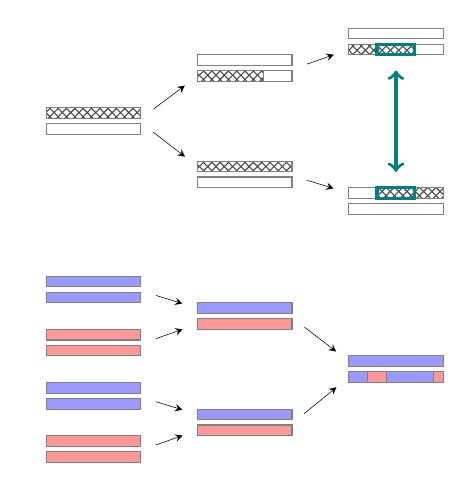
\begin{tikzpicture}[yscale=0.09, xscale=0.12]

\tikzset{
pop1/.style={fill=blue!40,draw=black!50},
pop2/.style={fill=red!40,draw=black!50},
ibd/.style={pattern=crosshatch,pattern color=black!70,draw=black!50},
nonibd/.style={fill=white,draw=black!50},
inherit/.style={->,>=stealth,ultra thin,shorten <=2mm,shorten >=2mm,very thin},
recomb/.style={thick,draw=black!70}
}

% Nodes
\node (hapx) at (1,0) {};
\node (hapy) at (0,1.5) {};
\node (hapxy) at ($10*(hapx) + (hapy)$) {};

\node (gen1) at (0,0) {};
\node (gen2) at ($8*(hapx) + 0*(hapx)$) {};
\node (gen3) at ($8*(hapx) + 8*(hapx)$) {};

\node (ind1gen3) at ($(gen3) + (0,0)$) {};
\node (indsep) at ($5*(hapy)$) {};

\node (ind1gen2) at ($(gen2) + 1*(indsep)$) {};
\node (ind2gen2) at ($(gen2) - 1*(indsep)$) {};

\node (ind1gen1) at ($(gen1) + 1.5*(indsep)$) {};
\node (ind2gen1) at ($(gen1) + 0.5*(indsep)$) {};
\node (ind3gen1) at ($(gen1) - 0.5*(indsep)$) {};
\node (ind4gen1) at ($(gen1) - 1.5*(indsep)$) {};

\node (chr1) at ($0.25*(hapy)$)  {};
\node (chr2) at ($-1.25*(hapy)$) {};


% Haplotypes

\filldraw[pop1] ($(gen1) + (ind1gen1) + (chr1)$) rectangle +(hapxy);
\filldraw[pop1] ($(gen1) + (ind1gen1) + (chr2)$) rectangle +(hapxy);

\filldraw[pop2] ($(gen1) + (ind2gen1) + (chr1)$) rectangle +(hapxy);
\filldraw[pop2] ($(gen1) + (ind2gen1) + (chr2)$) rectangle +(hapxy);

\filldraw[pop1] ($(gen1) + (ind3gen1) + (chr1)$) rectangle +(hapxy);
\filldraw[pop1] ($(gen1) + (ind3gen1) + (chr2)$) rectangle +(hapxy);

\filldraw[pop2] ($(gen1) + (ind4gen1) + (chr1)$) rectangle +(hapxy);
\filldraw[pop2] ($(gen1) + (ind4gen1) + (chr2)$) rectangle +(hapxy);


\filldraw[pop1] ($(gen2) + (ind1gen2) + (chr1)$) rectangle +(hapxy);
\filldraw[pop2] ($(gen2) + (ind1gen2) + (chr2)$) rectangle +(hapxy);

\filldraw[pop1] ($(gen2) + (ind2gen2) + (chr1)$) rectangle +(hapxy);
\filldraw[pop2] ($(gen2) + (ind2gen2) + (chr2)$) rectangle +(hapxy);


\filldraw[pop1] ($(gen3) + (ind1gen3) + (chr1)$) rectangle +(hapxy);
\fill[pop1] ($(gen3) + (ind1gen3) + (chr2)$) rectangle +(hapxy);
\fill[pop2] ($(gen3) + (ind1gen3) + (chr2)+ 2*(hapx)$) rectangle ($(gen3) + (ind1gen3) + (chr2)+ (hapxy)$);
\fill[pop1] ($(gen3) + (ind1gen3) + (chr2)+ 4*(hapx)$) rectangle ($(gen3) + (ind1gen3) + (chr2)+ (hapxy)$);
\fill[pop2] ($(gen3) + (ind1gen3) + (chr2)+ 9*(hapx)$) rectangle ($(gen3) + (ind1gen3) + (chr2)+ (hapxy)$);
%\draw ($(gen3) + (ind1gen3) + (chr2)$) rectangle +(hapxy);


% Copying lines

\node (startline) at ($-1*(hapx) + 0.5*(hapy)$) {};
\node (chrdiff) at ($(chr1) - (chr2)$) {};


% Arrows
\draw[inherit] ($(gen1) + (ind1gen1) + (chr2) + 10*(hapx) + 0.75*(chrdiff)$) -- ($(gen2) + (ind1gen2) + (chr1) + 0.5*(hapy)$);
\draw[inherit] ($(gen1) + (ind2gen1) + (chr2) + 10*(hapx) + 0.75*(chrdiff)$) -- ($(gen2) + (ind1gen2) + (chr2) + 0.5*(hapy)$);
\draw[inherit] ($(gen1) + (ind3gen1) + (chr2) + 10*(hapx) + 0.75*(chrdiff)$) -- ($(gen2) + (ind2gen2) + (chr1) + 0.5*(hapy)$);
\draw[inherit] ($(gen1) + (ind4gen1) + (chr2) + 10*(hapx) + 0.75*(chrdiff)$) -- ($(gen2) + (ind2gen2) + (chr2) + 0.5*(hapy)$);

\draw[inherit] ($(gen2) + (ind1gen2) + (chr2) + 10*(hapx) + 0.75*(chrdiff)$) -- ($(gen3) + (ind1gen3) + (chr1) + 0.5*(hapy)$);
\draw[inherit] ($(gen2) + (ind2gen2) + (chr2) + 10*(hapx) + 0.75*(chrdiff)$) -- ($(gen3) + (ind1gen3) + (chr2) + 0.5*(hapy)$);


%%%%%%%%%%%%%%%%%%%%%
% Identity-by-descent
% Nodes
\node (hapx) at (1,0) {};
\node (hapyIBD) at (0,+35.0) {};
%\node (hapxy) at ($10*(hapx) + (hapy)$) {};

%\node (gen1) at (0,0) {};
%\node (gen2) at ($8*(hapx) + 0*(hapx)$) {};
%\node (gen3) at ($8*(hapx) + 8*(hapx)$) {};

%\node (indsep) at ($5*(hapy)$) {};
\node (ind1gen3) at ($(gen3) + 1.5*(indsep)$) {};
\node (ind2gen3) at ($(gen3) - 1.5*(indsep)$) {};

\node (ind1gen2) at ($(gen2) + 1*(indsep)$) {};
\node (ind2gen2) at ($(gen2) - 1*(indsep)$) {};

\node (ind1gen1) at ($(gen1) + 0*(indsep)$) {};

\node (chr1) at ($0.25*(hapy) + (hapyIBD)$)  {};
\node (chr2) at ($-1.25*(hapy)+ (hapyIBD)$) {};

% Haplotypes
\filldraw[ibd] ($(gen1) + (ind1gen1) + (chr1)$) rectangle +(hapxy);
\filldraw[nonibd] ($(gen1) + (ind1gen1) + (chr2)$) rectangle +(hapxy);

\filldraw[nonibd] ($(gen2) + (ind1gen2) + (chr1)$) rectangle +(hapxy);
\filldraw[ibd] ($(gen2) + (ind1gen2) + (chr2)$) rectangle +(hapxy);
\filldraw[nonibd] ($(gen2) + 7*(hapx) + (ind1gen2) + (chr2)$) rectangle ($(gen2) + (ind1gen2) + (chr2) + (hapxy)$);

\filldraw[ibd] ($(gen2) + (ind2gen2) + (chr1)$) rectangle +(hapxy);
%\filldraw[ibd] ($(gen2) + 3*(hapx) + (ind2gen2) + (chr1)$) rectangle ($(gen2) + (hapxy) + (ind2gen2) + (chr1)$);
\filldraw[nonibd] ($(gen2) + (ind2gen2) + (chr2)$) rectangle +(hapxy);

\filldraw[nonibd] ($(gen3) + (ind1gen3) + (chr1)$) rectangle +(hapxy);
\filldraw[ibd] ($(gen3) + (ind1gen3) + (chr2)$) rectangle +(hapxy);
\filldraw[nonibd] ($(gen3) + 7*(hapx) + (ind1gen3) + (chr2)$) rectangle ($(gen3) + (ind1gen3) + (chr2) + (hapxy)$);

\filldraw[nonibd] ($(gen3) + (ind2gen3) + (chr1)$) rectangle +(hapxy);
\filldraw[ibd] ($(gen3) + 3*(hapx) + (ind2gen3) + (chr1)$) rectangle ($(gen3) + (hapxy) + (ind2gen3) + (chr1)$);
\filldraw[nonibd] ($(gen3) + (ind2gen3) + (chr2)$) rectangle +(hapxy);

% Arrows
\draw[inherit] ($(gen1) + (ind1gen1) + (chr1) + 10*(hapx) + 0*(chrdiff)$) -- ($(gen2) + (ind1gen2) + (chr2) + 0.5*(hapy)$);
\draw[inherit] ($(gen1) + (ind1gen1) + (chr1) + 10*(hapx) - 0.25*(chrdiff)$) -- ($(gen2) + (ind2gen2) + (chr1) + 0.5*(hapy)$);

\draw[inherit] ($(gen2) + (ind1gen2) + (chr2) + 10*(hapx) + 0.75*(chrdiff)$) -- ($(gen3) + (ind1gen3) + (chr2) + 0.5*(hapy)$);
\draw[inherit] ($(gen2) + (ind2gen2) + (chr1) + 10*(hapx) - 0.25*(chrdiff)$) -- ($(gen3) + (ind2gen3) + (chr1) + 0.5*(hapy)$);

% IBD highlight.
\draw[color=teal,very thick] ($(gen3) + (ind1gen3) + (chr2) + 3*(hapx)$) rectangle +($4*(hapx) + (hapy)$);
\draw[color=teal,very thick] ($(gen3) + (ind2gen3) + (chr1) + 3*(hapx)$) rectangle +($4*(hapx) + (hapy)$);
\draw[color=teal,very thick,<->,shorten <=2mm,shorten >=2mm] ($(gen3) + (ind1gen3) + (chr2) + 5*(hapx)$) -- ($(gen3) + (ind2gen3) + (chr1) + 5*(hapx) + (hapy)$) ; 

% Labels
%\node (lab1) at ($(gen1) + 2.5*(indsep) + 0.5*(hapxy) - (hapyIBD)$) {\scriptsize $\texttt{Generation 0}$};
%\node (lab2) at ($2*(gen2) + 2.5*(indsep) + 0.5*(hapxy) - (hapyIBD)$) {\scriptsize $\texttt{Generation 1}$};
%\node (lab3) at ($4*(gen2) + 2.5*(indsep) + 0.5*(hapxy) - (hapyIBD)$) {\scriptsize $\texttt{Generation 2}$};

\end{tikzpicture}

%\end{center}
\end{minipage}\hspace{1cm}\begin{minipage}{.45\linewidth}
\flushright
{\bf\magenta{Identity-by-descent (IBD):}}\\
Which segments came from the same ancestral chromosome?
\vspace{15mm}

{\bf\magenta{Local ancestry (LA):}}\\
Which segments came from ancestors in a given population?
\end{minipage}
\end{frame}

\begin{frame}
\frametitle{IBD and LA can be extracted from tree sequences}
%\begin{center}
\begin{minipage}{.33\linewidth}
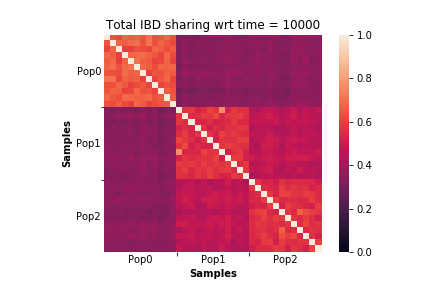
\includegraphics[scale=.3]{pics/kinships-10000.png}
\end{minipage}\begin{minipage}{.33\linewidth}
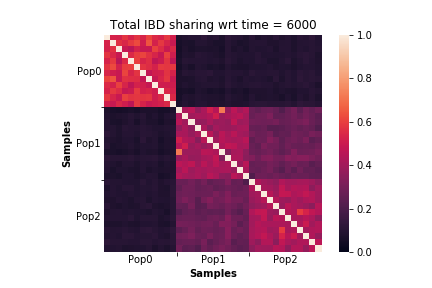
\includegraphics[scale=.3]{pics/kinships-6000.png}
\end{minipage}\begin{minipage}{.33\linewidth}
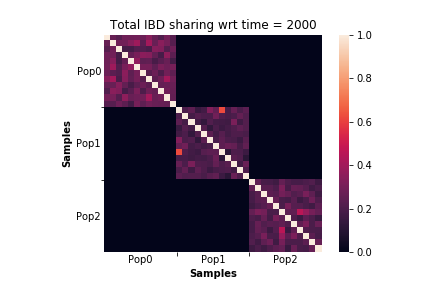
\includegraphics[scale=.3]{pics/kinships-2000.png}
\end{minipage}

\vspace{5mm}


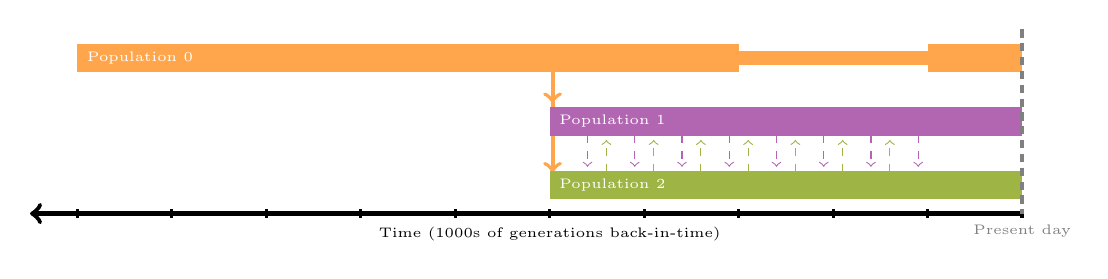
\begin{tikzpicture}[node distance=5mm and 5mm,xscale=1.2,yscale=0.18,rotate=90]

\tikzset{greynode/.style={font=\footnotesize,node distance=1cm and 1 cm,fill=black!10,draw=black!30,inner sep=0pt,minimum size=3.5mm,shape=circle},
mutations/.style={shape=starburst,fill=red!50!blue,inner sep=0.8pt,starburst points=11,starburst point height=.2cm},
pop0/.style={orange!70},pop1/.style={violet!60},pop2/.style={olive!70!green!70!white}}

% Nodes
\node (origin) at (0,0){};
\node (pop0) at (10,0){};
\node (pop1) at (5.5,0){};
\node (pop2) at (1,0){};
\node (popwidth) at (2,0){};

% Axis
\node (leftAx) at (-1,0) {};
\draw[line width=.6mm,->] (-1,0) -- +(0, 10.5);
\foreach \y in {0, 1, 2, 3, 4, 5, 6, 7, 8, 9, 10} \draw[very thick] ($(leftAx) + (-0.3, \y)$) -- ($(leftAx) + (0.3, \y)$); % tick marks
%\node[anchor=east] at ($(leftAx)$) {0}; \node[anchor=east] at ($(leftAx) + (0,5)$) {5};
\node[anchor=north] (leftLabel) at ($(leftAx) + (-0.3,5)$) {\tiny $\textrm{Time (1000s of generations back-in-time)}$};

% Migrations
\foreach \y in {0.5,1,1.5,2,2.5,3,3.5,4} \draw[pop1,dashed,->] ($(.1,.1) + (leftAx) + (0,\y + .5)+(pop1) $) -- +(-2.3,0);
\foreach \y in {1,1.5,2,2.5,3,3.5,4} \draw[pop2,dashed,->] ($(-.1,-.1) + (leftAx) + (0,\y + .5)+(pop2) + (popwidth)$) -- +(2.3,0);
\draw[pop0, ->, line width=.5mm] ($(.1,0) + (leftAx) + (0,4.97)+(pop0) $) -- +(-2.3,0);
\draw[pop0, ->, line width=.5mm] ($(.1,0) + (leftAx) + (0,4.97)+(pop0) $) -- +($-3*(2.4,0)$);

% Populations
\foreach \x in {0} \fill[pop\x] ($(leftAx) + (pop\x)$) -- ++(0,10) -- ++(2, 0) -- ++(0, -10) -- cycle;
\foreach \x in {1, 2} \fill[pop\x] ($(leftAx) + (pop\x)$) -- ++(0,5) -- ++(2, 0) -- ++(0, -5) -- cycle;
\foreach \x in {0} \node[right,white] (label\x) at ($(leftAx) + (pop\x) + (1, 10)$) {{\tiny Population \x}};
\foreach \x in {1,2} \node[right,white] (label\x) at ($(leftAx) + (pop\x) + (1, 5)$) {{\tiny Population \x}};


% Times
\draw[densely dashed,color=gray,very thick] (12,0) -- (-1,0) node[below] {\tiny Present day} ;

% White squares over pop0 bottleneck areas.
\fill[white] ($(leftAx) + 0.9*(pop0) + (0,1)$) -- ++($0.15*(pop0)$) -- ++(0,2) -- ++($-0.15*(pop0)$) -- cycle;
\fill[white] ($(leftAx) + 1.1*(pop0) +(popwidth) + (0,1)$) -- ++($-0.15*(pop0)$) -- ++(0,2) -- ++($0.15*(pop0)$) -- cycle;

\end{tikzpicture} 

%\end{center}
\end{frame}

\begin{frame}
\frametitle{Future work: what can we infer with this information?}
\begin{minipage}{.45\linewidth}
\begin{center}
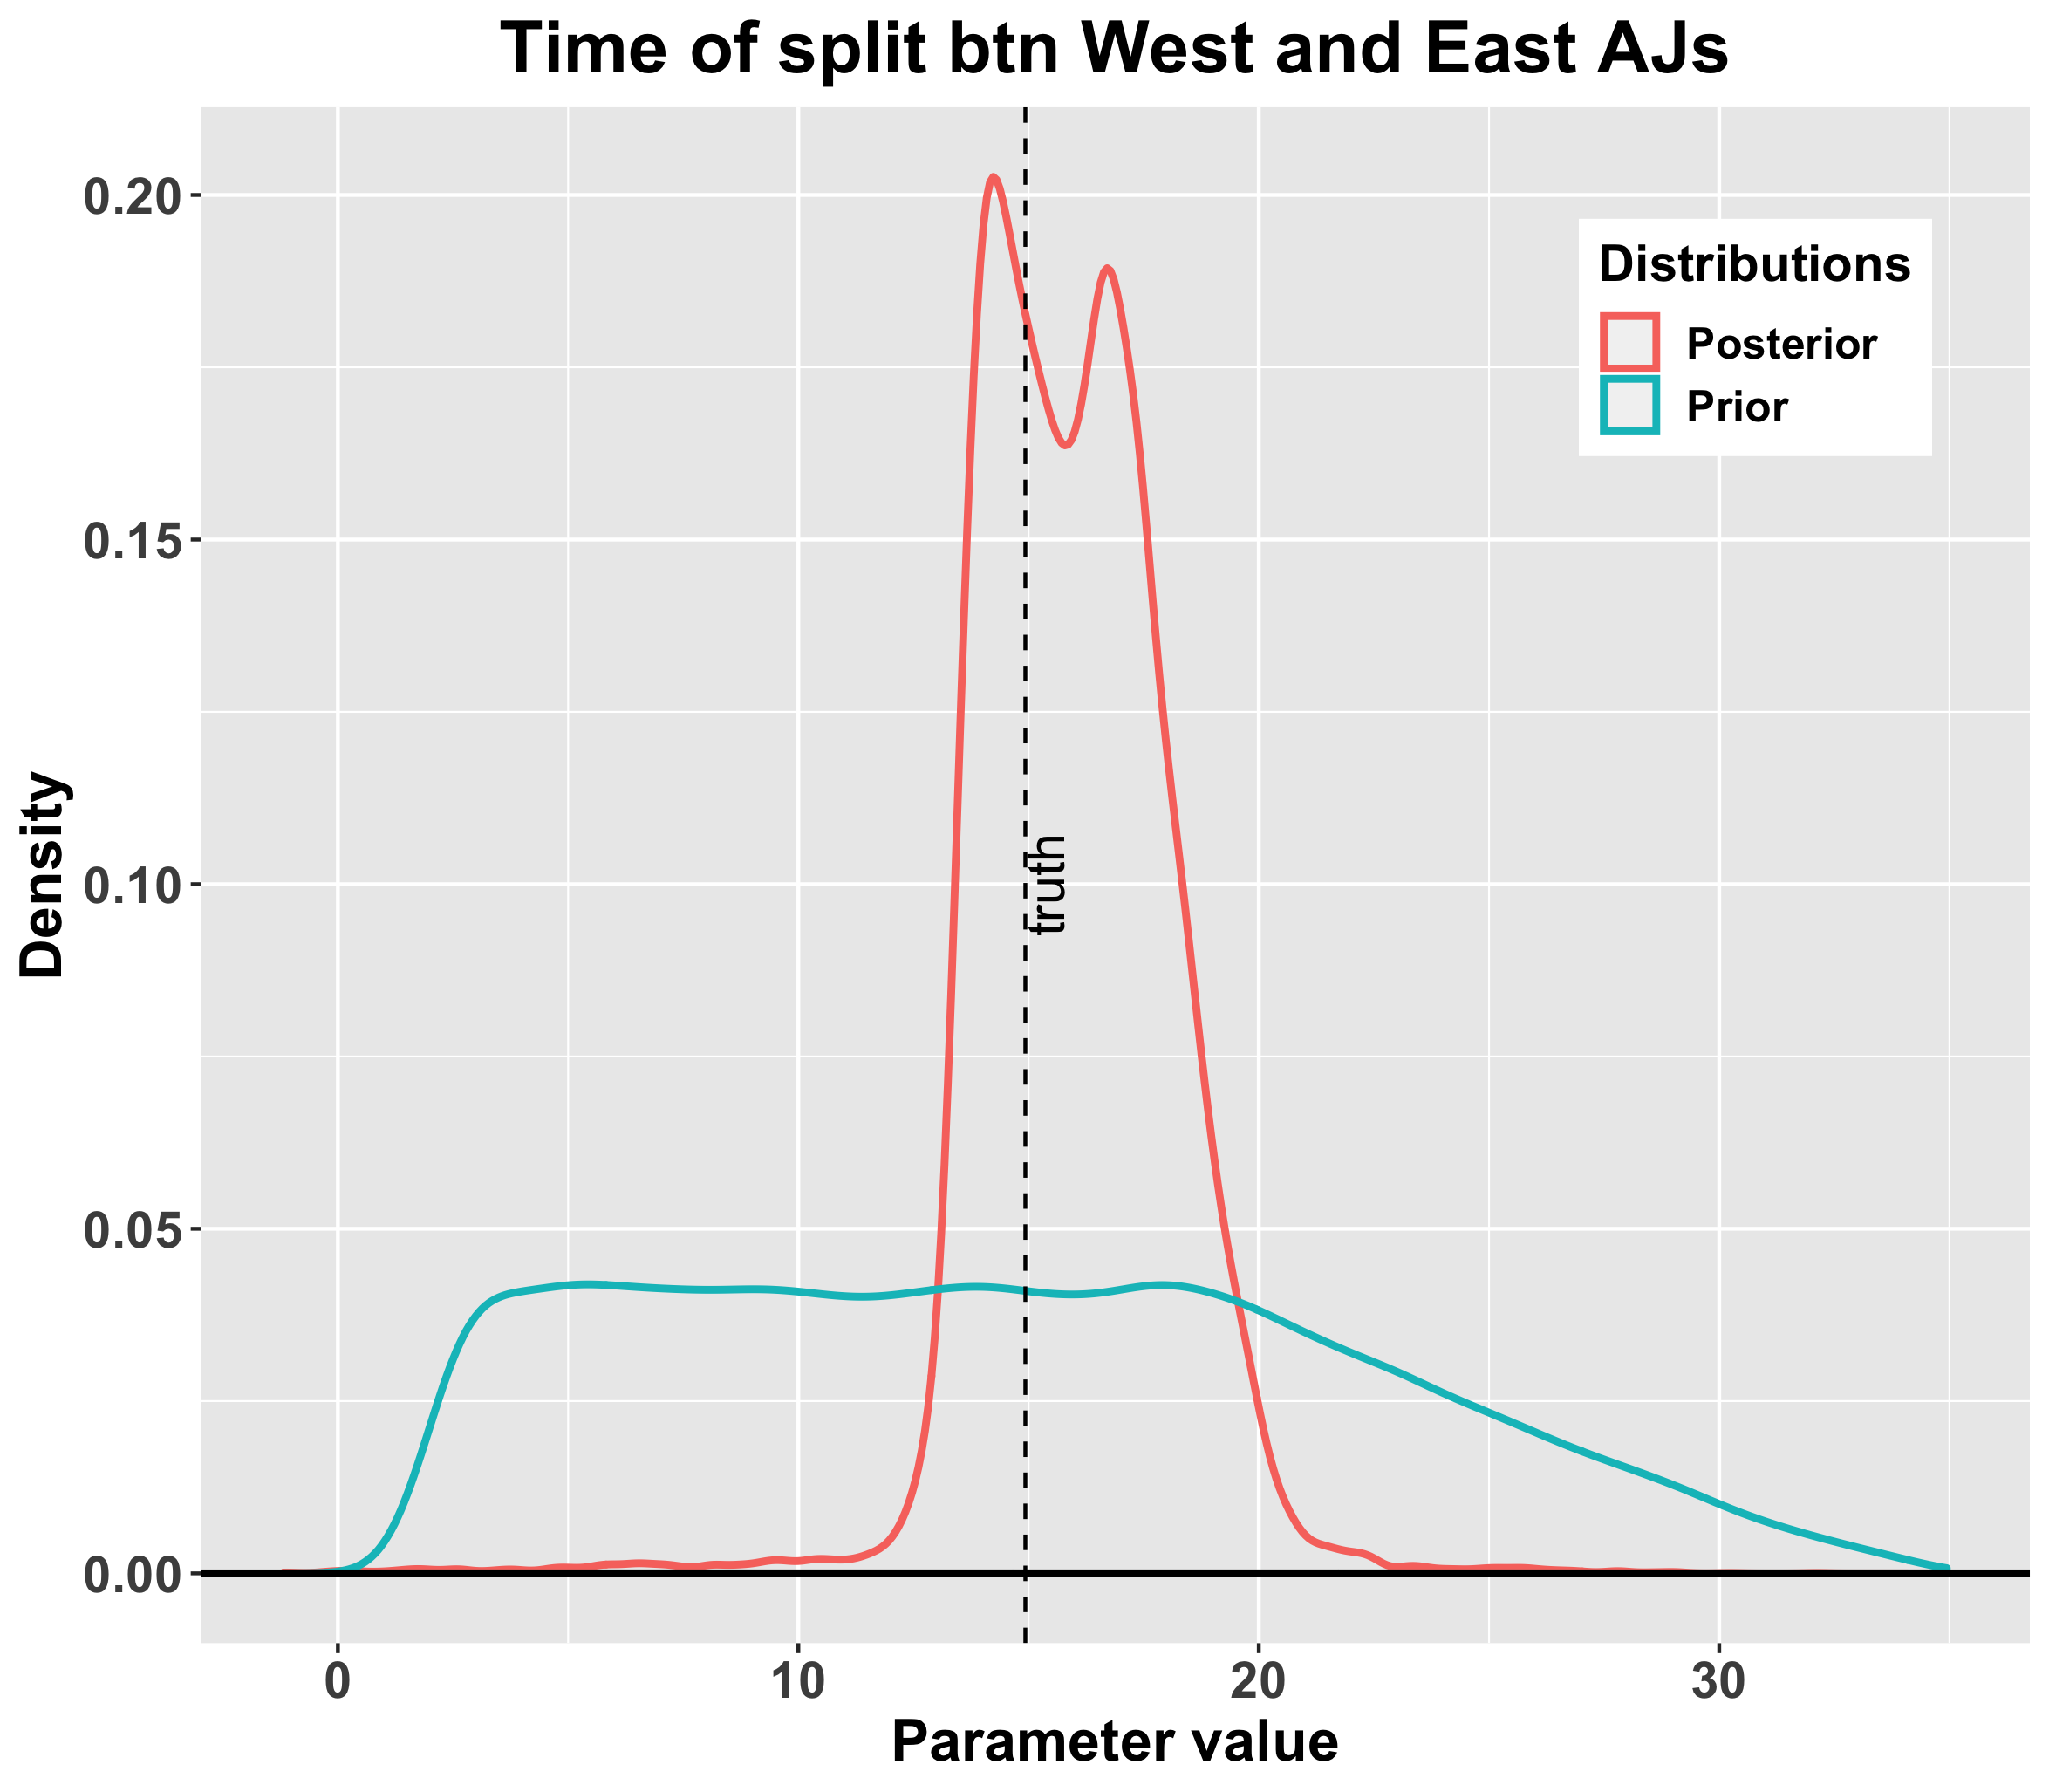
\includegraphics[scale=.06]{pics/abc-ibd-4.png}
\end{center}
\end{minipage}\begin{minipage}{.5\linewidth}
\centering
See poster $\# 32$ tonight!

\begin{minipage}{.25\linewidth}

\includegraphics[scale=.3]{pics/unimelb-logo.jpg}
\end{minipage}\begin{minipage}{.25\linewidth}

\includegraphics[scale=.3]{pics/tskit-logo.png}
\end{minipage}
\flushright
\texttt{https://tskit.readthedocs.io/}
\end{minipage}
\end{frame}

\end{document}